\documentclass[journal,twocolumn]{IEEEtran}
\usepackage{cite}
% *** GRAPHICS RELATED PACKAGES ***
\usepackage[pdftex]{graphicx}
\usepackage{authblk}
\usepackage{booktabs}
\usepackage{xcolor}
\usepackage{tikz}
\usepackage[utf8]{inputenc}
\usepackage[T1]{fontenc}

\usetikzlibrary{arrows.meta, positioning, calc}

%\graphicspath{{../pdf/}{../jpeg/}}
\DeclareGraphicsExtensions{.pdf,.jpeg,.png}

% *** PDF, URL AND HYPERLINK PACKAGES ***
\usepackage[hyphens]{url}
\usepackage[hidelinks]{hyperref}
% correct bad hyphenation here
\hyphenation{op-tical net-works semi-conduc-tor}

% \usepackage{draftwatermark}
% \SetWatermarkText{DRAFT}
% \SetWatermarkScale{1}

\usepackage{easyReview}

\begin{document}
\title{Analyzing Trade-offs in Refresh, Frequency, and Isolation Approaches to RowHammer Mitigations}
\author{\IEEEauthorblockN{Haorong Xu}\\
		\textit{British International Course Centre (96661)}\\
		Guangzhou, China \\
		Xu.Haorong@scagz.com}
\maketitle

\begin{abstract}
	RowHammer is a critical DRAM vulnerability that enables bit-flips via rapid row activations and compromises data integrity. As the storage density of DRAM scales, the RowHammer effect worsens, rendering existing mitigations increasingly costly and ineffective. This study surveys and systematizes major RowHammer mitigations, particularly those published after 2023, using the refresh-centric, frequency-centric, and isolation-centric taxonomy of Loughlin et al.
	
	Evaluation reveals that the the majority of mitigations are fundamentally unscalable against decreasing RowHammer threshold, while reactive mitigations are undermined by the RowPress attack variant. Furthermore, the timing side-channel inherent in access-pattern-dependent mitigations remains a critical yet underappreciated issue. By extending the Naseredini review to current literature and applying the failure mode framework of Jaleel et al. to refresh-centric mitigations in a uniform comparison, the analysis identifies the non-mutual-exclusivity of Loughlin's taxonomy. Finally, this study demonstrates an inherent conflict between robust security and operational efficiency, revealing that existing mitigations cannot concurrently optimize security determinism, storage density, and latency.
\end{abstract}

\begin{IEEEkeywords}
	DRAM, RowHammer, Microarchitecture Security
\end{IEEEkeywords}

\section{Introduction}

\IEEEPARstart{D}{ynamic} Random-Access Memory (DRAM) is a ubiquitous primary storage medium in computing systems. RowHammer attack\cite{Kim14} is a disturbance error that remains a significant threat to DRAM's security and reliability. It allows attackers to flip the bits of adjacent DRAM rows by frequently reading from a row. RowHammer structurally undermines memory isolation, a foundational security guarantee on which modern operating systems are built. Consequently, this enables malicious applications to compromise the availability, reliability, and confidentiality of computer systems. For example, \cite{Seaborn15} demonstrated that it is possible to escalate privilege by ``hammering" sensitive data entries in memory. The scaling of DRAM has exacerbated RowHammer: the RowHammer Threshold, the number of activations required to induce bit-flips falls as the storage density of DRAM continues to increase, as illustrated by Figure \ref{fig:threshold}. A lot of mitigations thought to be RowHammer-free were then defeated at low RowHammer thresholds\cite{Orosa21}.

Several surveys have synthesized the RowHammer mitigation literature. However, existing surveys primarily classify mitigations by implementation level (e.g. Hardware-based versus Software-based). This study adopts a different analytical lens, focusing on the mechanisms and failure modes of mitigations. It builds on Loughlin's taxonomy\cite{Loughlin21}, dividing mitigations into \textit{Refresh-Centric, Frequency-Centric}, and \textit{Isolation-Centric}.

This study leverages and critiques Loughlin's taxonomy and analyzes each group of mitigations in detail. Specifically, this study adopts Jaleel's\cite{Jaleel24} framework to assess trackers used in refresh-centric mitigations, which are data structures responsible for monitoring row activations. This framework sees in-DRAM trackers as governed by three policies --- insertion  (determining which rows enter the tracker), eviction (managing entry replacement), and mitigation (deciding rows to preventively mitigate).

The cross-category analysis leads to the conclusion of a trilemma: all current mitigations fail to achieve deterministic-security, space-efficiency, and low latency simultaneously. Sources were identified through searches of Google Scholar, IEEE Xplore, and ACM Digital Library using the terms \textit{RowHammer}, \textit{DRAM Disturbance Error}, and \textit{Mitigation}. Articles published in 2023 and onward are prioritized. As for prior works, this study refers to Naseredini's comprehensive review of RowHammer and its mitigations as an index\cite{Naseredini23}.

\section{Background}\label{sec:bg}

\subsection{DRAM Organization}
\begin{figure}[h]
	\centering
	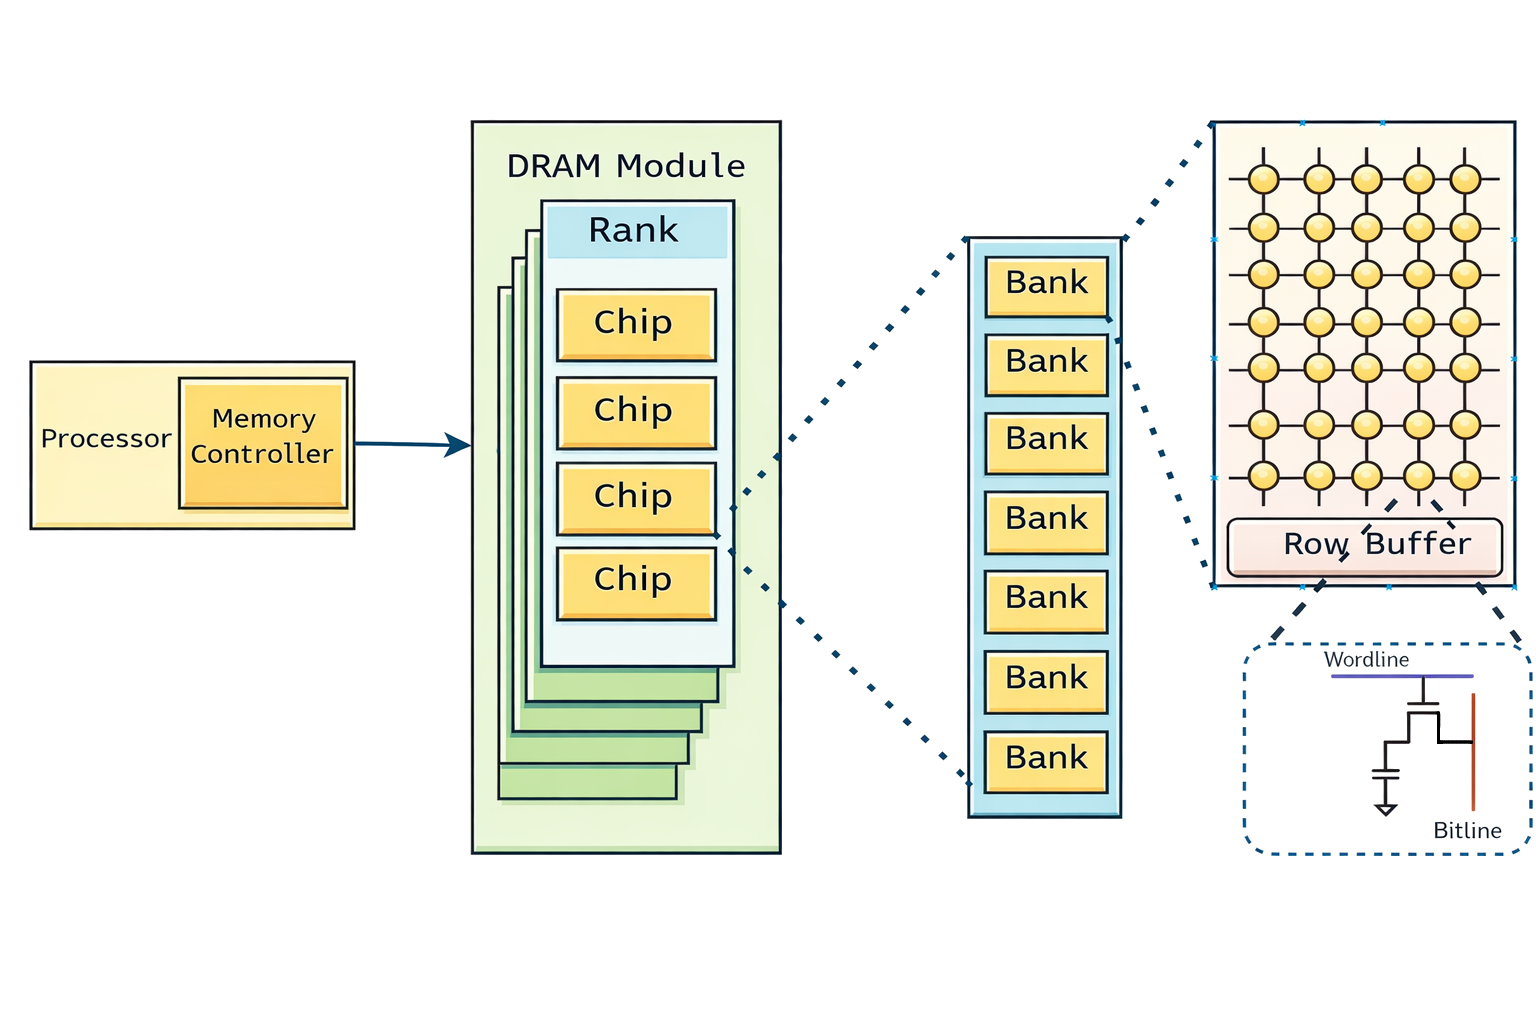
\includegraphics[width=\columnwidth]{drambanks_colored.png}
	\caption{High-level DRAM structure}\label{fig:dramstruct}
\end{figure}

Dynamic Random-Access Memory (DRAM) is the most common storage medium used by processors because of its high storage density.
Fig.\ref{fig:dramstruct} illustrates the overall structure of a modern DRAM module. A DRAM module consists of multiple DRAM chips, each featuring several DRAM banks that can be accessed concurrently. Within each bank there are subarrays of densely packed DRAM cells, in which a row of DRAM cells is connected through a \textit{wordline} and a \textit{bitline} joins all cells in a column. Each subarray is isolated from the others since they do not share bitlines. A DRAM cell consists of an access transistor and a capacitor. The bit is stored as electric charge in the capacitor, where the cell represents ``0" when the capacitor is uncharged and ``1" when it is fully charged. When the wordline is activated by putting a voltage on it, all access transistors in the corresponding row are enabled, which allows the charge in the capacitor to be carried onto the bitline. All bitlines eventually connect to a \textit{row buffer} at the edge of the subarray, a DRAM row acting as a cache of the most recently accessed row.

To read from a DRAM row, the system physical address first needs to be translated into a logical DRAM address, which specifies banks, rows, columns, etc., and the translation is usually carried out by a programmable \textit{memory controller}\cite{DRAMMapping}. The logical address is then translated into an internal address, which is a feature used by manufacturers to internally remap bad rows to other locations to tolerate faults. Next, the row is activated, and the row being read is loaded to the row buffer as charge in capacitors storing ``1" flows into the row buffer via the bitlines. Subsequent read and write operations can be carried out on the row buffer. Since charge in capacitors inherently flows out over time, data has to be written back to the capacitors afterward.

Capacitors inherently leak charge over time. Therefore, the memory controller periodically performs \textit{Refresh} operations to retain data, which will read and rewrite all data in the DRAM so the capacitors are again fully charged. Specifically, the memory controller issues a refresh instruction (REF) every $t_{REFI}$, and any row is guaranteed to be refreshed within $t_{REFW}$ (Refresh Window).

\subsection{RowHammer}\label{sec:bg-rowhammer}

RowHammer refers to a DRAM vulnerability where by changing the voltage in a wordline repeatedly, an attacker can reliably induce bit-flips in nearby rows. In 2014, Kim et al\cite{Kim14}. first observed that, by frequently toggling wordlines, nearby cells leak their charge at an accelerated rate so that the cells cannot retain their charge before $t_{REFW}$, leading to bits flipped from 1 to 0. A previous study\cite{Walker21} attributes circuit-level disturbance error primarily to two electromagnetic interference phenomena:  \textit{Eletron Injection and Capture}, and \textit{Capacitive Crosstalk}. \cite{Cojocar20} also demonstrated that the RowHammer effect exhibits a spatial locality, meaning the number of bit-flips in a row is positively correlated to its distance from the \textit{aggressor row} (\textit{i.e.} the row that is being "hammered"), which leads to the term \textit{blast radius}, the maximum distance an aggressor row can affect.

\begin{figure}[h]
	\centering
	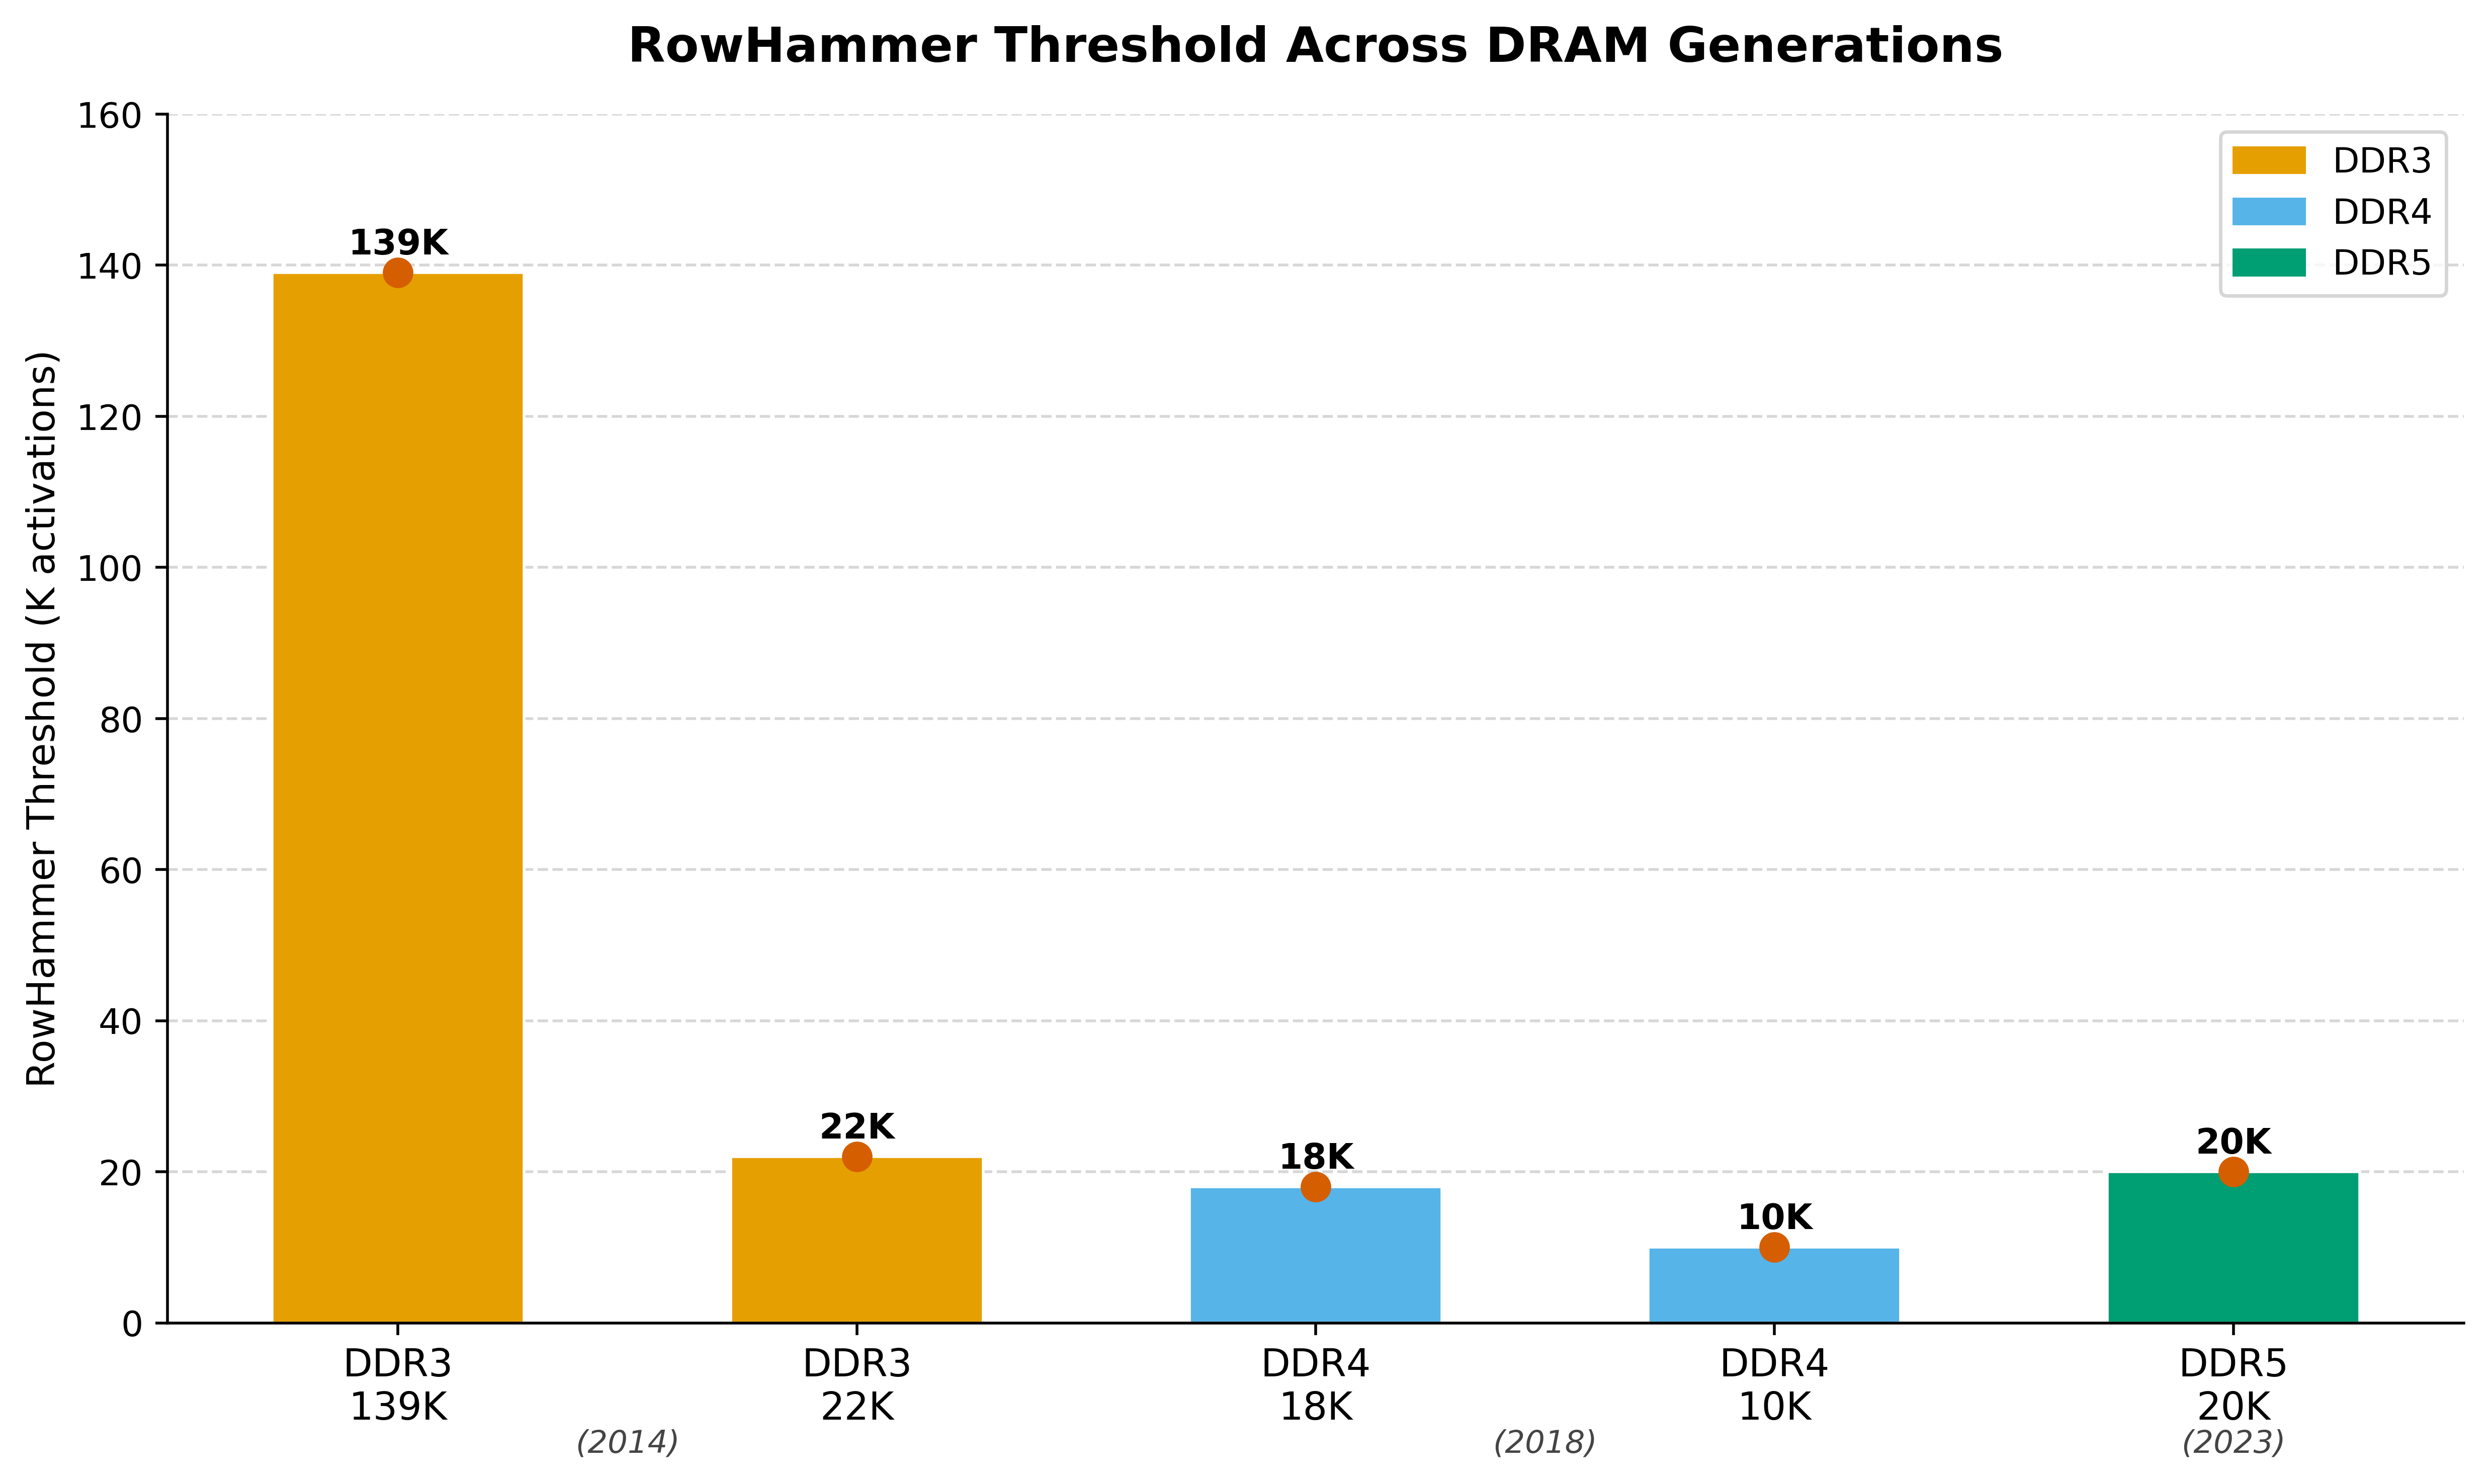
\includegraphics[width=\columnwidth]{rowhammer_thres.png}
	\caption{The RowHammer Threshold $T_{RH}$ across different generations of DRAM (Data from \cite{Saxena24,Gloor25}). Overall, $T_{RH}$ continues to decrease, and the rebound in DDR5 is attributed to built-in RowHammer mitigation in DDR5 chips\cite{Gloor25}. DDR5 would have a $T_{RH}$ lower than 10k without it.}\label{fig:threshold}
\end{figure}

To launch a RowHammer attack, the aggressor rows must be activated enough times before victim rows are refreshed (\textit{i.e.} within $t_{REFI}$) such that the accumulated disturbance induces bit-flips. As mentioned earlier, refreshing would fully charge all capacitors in a row, which offsets the attacker's effort. Therefore, refreshing victim rows before they experience bit-flips can be used as a defense to RowHammer (further discussed in \ref{sec:refresh-centric}).

Unfortunately, the RowHammer vulnerability is worsening over time. As the storage density of DRAM continues to grow, the number of activations required to induce a bit-flip, denoted as $T_{RH}$ (the RowHammer Threshold), has been continuously decreasing over the last decade, as illustrated by Fig.\ref{fig:threshold}. As DRAM cell size and cell-to-cell spacing shrink, they are more susceptible to the aforementioned interference. In today's most prevalent DRAM devices, $T_{RH}$ is as low as 10k to 20k. This trend poses severe risks to new DRAM devices because it is easier to induce bit-flips with fewer activation count, and an aggressor row can affect more potential victims.

\begin{figure}[h]
	\centering
	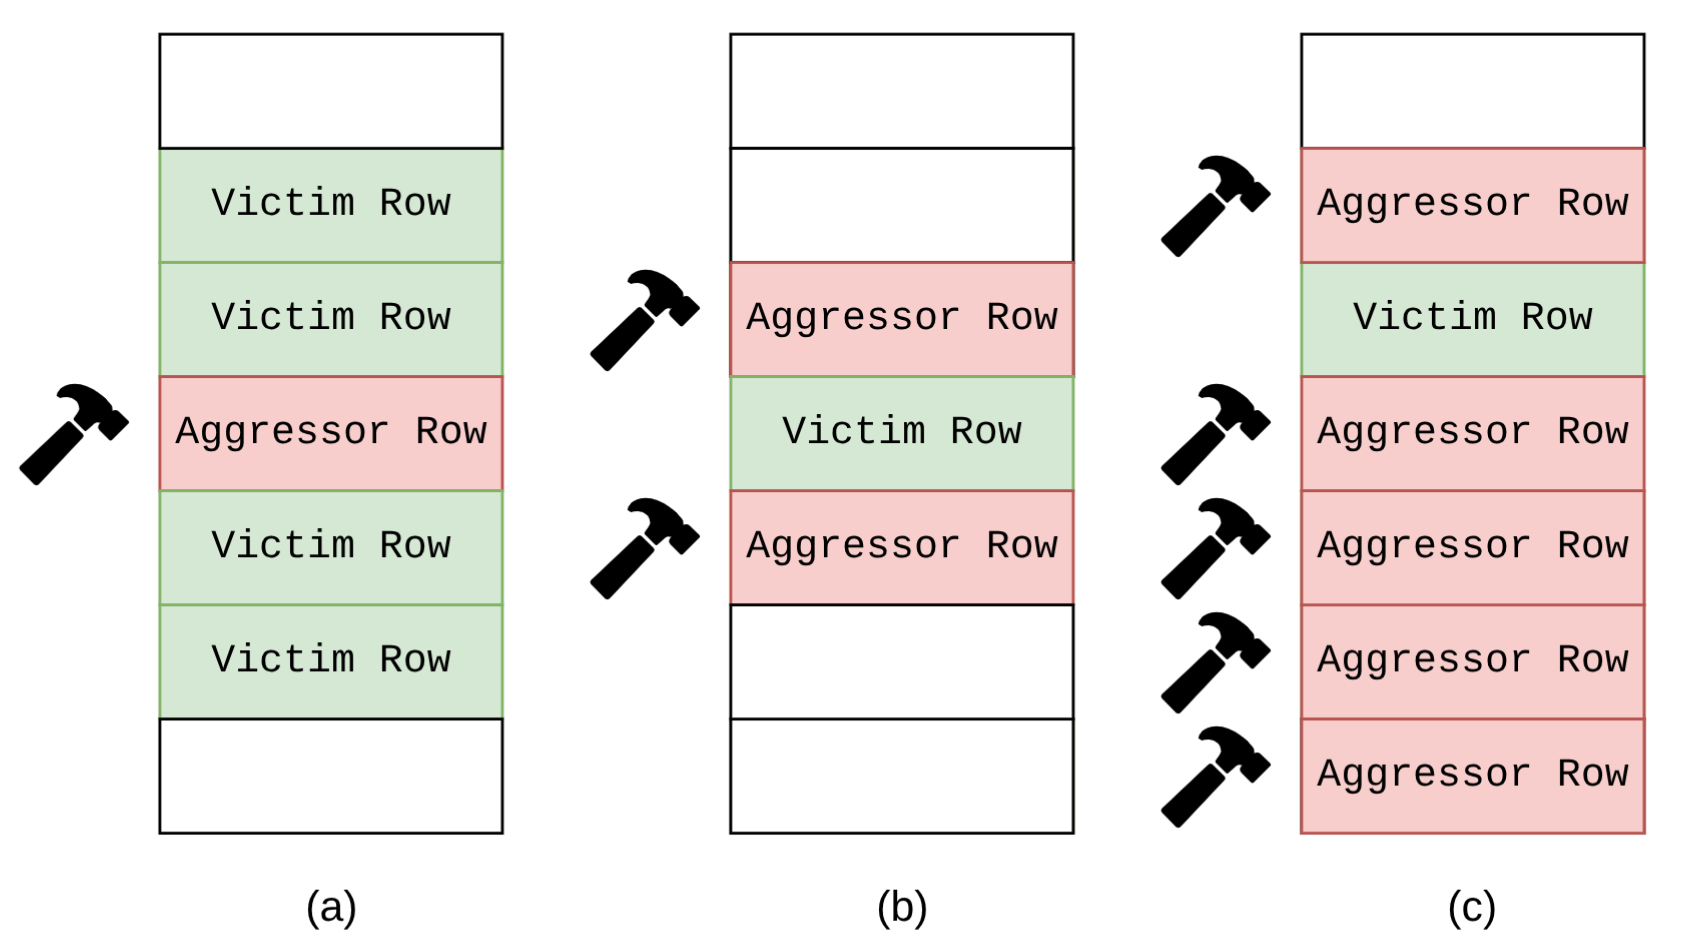
\includegraphics[width=\columnwidth]{sides.png}
	\caption{(a) Single-sided RowHammer: only one row is hammered, and the rows within its blast radius are affected. (b) Double-sided RowHammer: two aggressor rows sandwich a victim row in between. (c) Many-sided RowHammer: many rows hammered simultaneously.}\label{fig:sided}
\end{figure}

RowHammer poses a severe security risk to computer systems, as it disrupts \textit{memory isolation}, where accessing a row alters data stored in nearby rows. Many works have demonstrated the far-reaching impact of RowHammer. For instance, \cite{Seaborn15} illustrated that by inducing bit-flips in \textit{Page Table Entry}, a data structure used by the OS to translate virtual memory address to physical memory address, an attacker can gain read and write permission to arbitrary location in the memory and escalate privilege. Other works have shown that it is capable of leaking confidential data, such as Deep Neural Networks (DNNs) weights\cite{Rakin22}, digital signature key\cite{Mus23}, and other processes' memory\cite{Kwong20}. Although no in-the-wild attacks have been reported, a recent survey by Heckel et al.\cite{Heckel26} shows that $12.5\%$ of the tested DRAM are vulnerable to fully automated RowHammer attacks, confirming that RowHammer remains a practical and scalable attack vector. 

Over the last decade, many mitigations have been proposed and defeated. Some sophisticated variants manipulate the \textit{access pattern}, defined as the sequence, frequency, and timing of memory access, to bypass mitigations. For instance, while the original RowHammer attack only hammers one row, subsequent double-sided attack\cite{Seaborn15} and many-sided attack\cite{Frigo20} leverages complex spatial patterns to amplify disturbance or overwhelm trackers. This will be discussed more in-depth in section \ref{sec:insertion}.

\subsection{Previous Works}\label{sec:prev-work}

RowHammer has been heavily researched since its first appearance, and many mitigation strategies have been proposed accordingly. Many works have attempted to synthesis the knowledge in the field (e.g. \cite{Naseredini23,Loughlin21,Zhang24,Kim25,MutluKim20,Mutlu23,Mutlu23_2}), and some tried to establish a uniform taxonomy for classifying RowHammer mitigations to provide insight for future research. A popular one is based on implementation level, dividing mitigations into either software-based or hardware-based. However, these two categories are too broad, and some recent works (e.g.\cite{Ojha25}) have employed a software-hardware co-design approach, blurring the line between these two categories.

The present work instead adopts the taxonomy proposed by Loughlin et al.\cite{Loughlin21}: \textit{isolation-centric, frequency-centric,} and \textit{refresh-centric}. Unlike the conventional taxonomy that classifies defenses according to the implementation level, this framework presents three categories which align with the physical conditions that can lead to disturbance errors: spatial proximity of aggressor and victim rows, frequent activation of aggressor rows, and victim rows not being refreshed before flipping, respectively. By focusing on functional mechanisms, it sheds light on why many mitigation strategies share similar \textit{failure mode}, the way in which a defense fails, and their performance tradeoffs.

Building on the survey by Naseredini\cite{Naseredini23} which covers mitigations up to 2023, this work comprehensively classifies and evaluates major RowHammer mitigations with an emphasis on the analysis to works published from 2023 onward. By breaking down each category of mitigations to analyze their failure modes and tradeoffs, it provides insights into building fundamentally robust and efficient mitigations for future studies. 

\section{RowHammer Mitigations}\label{sec:mitigation}

\subsection{Refresh-Centric}\label{sec:refresh-centric}

\begin{table*}
	\centering
	\caption{Stateful Refresh-Centric Mitigations}\label{tab:refreshcomp}
	\def\arraystretch{1.1}
	\begin{tabular}{p{0.25\columnwidth}p{0.5\columnwidth}p{0.5\columnwidth}p{0.4\columnwidth}c}
		\toprule
		Mitigation & Insertion Policy & Eviction Policy & Mitigation Policy & Reference \\
		\midrule
		PRAC & Per-row Counting & N/A & When counters exceed a threshold & \cite{JESD79-5C}
		\\
		ARS & Misra-Gries Algorithm & Rows with lower access count evicted & Top-two aggressor rows & \cite{Kim23}
		\\
		CoMeT & Hashing based Count-Min Sketch & Random selection & Rows with access count higher than a threshold & \cite{Bostanci24}
		\\
		ARAR & Per-row counting & N/A & Per-row probabilistic & \cite{Demirseren24}
		\\
		PrIDE & Probabilistic sampling & FIFO & FIFO 
		& \cite{Jaleel24}
		\\
		CHaRM & Upon every ACT & Evict old rows when a hash collision occurs & Upon eviction and when counter hits a threshold & \cite{Hajiabadi25}
		\\
		CnC-PRAC & Upon every ACT & Evict rows that occupy most entries in the tracker (one entry per byte) & When the counter exceeds a threshold & \cite{Lin25}
		\\
		ABACuS & Per-row counting (shared counters) & N/A & When the counter exceeds a threshold & \cite{Olgun24} 
		\\
		RIAC & Per-row counting & N/A & When the counter exceeds a threshold. Then randomize the counter & \cite{Bostanci25}
		\\
		TPRAC & Per-row counting & N/A & Periodically mitigate most accessed row & \cite{Woo25}
		\\
		MIRZA & Per-subarray counting & N/A & Perform MINT\cite{Qureshi24} mitigation on any subarray whose access count exceeds a threshold & \cite{Taneja26}
		\\
		MoPAC & Per-row counting with probabilistic sampling & N/A & When counter exceed a threshold & \cite{Vittal25}
		\\
		\bottomrule
		\\
		\multicolumn{5}{p{2\columnwidth}}{This table contrasts stateful refresh-centric mitigations by their insertion policy, eviction policy, and mitigation policy. In the table, ACT stands for activation. Per-row counting mitigations have no eviction policy as counters are kept for every row and never evicted, so their eviction policy are marked as ``N/A", Not Applicable. FIFO policy refers to \textit{First In, First Out}, meaning rows that remain in the tracker array for the longest time are evicted or mitigated first.}
	\end{tabular}
\end{table*}

\begin{figure}[h]
	\centering
	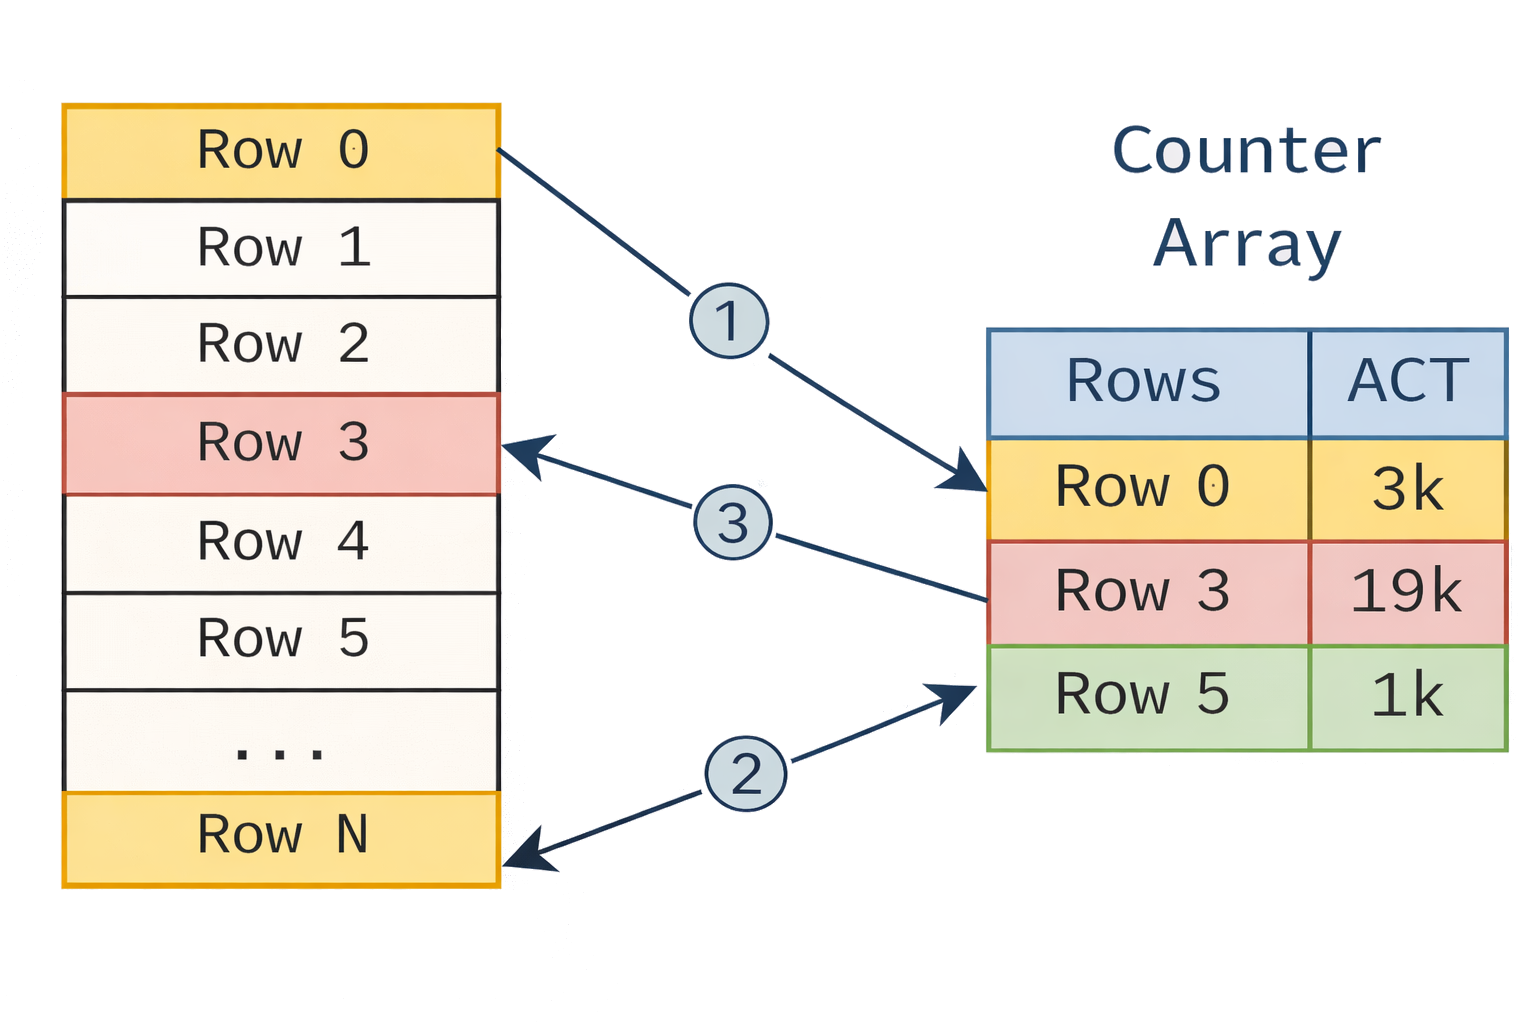
\includegraphics[width=\columnwidth]{refresh-centric_colored.png}
	\caption{Stateful refresh-centric mitigations are centered around three polices. 1. Insertion. 2. Eviction. 3. Mitigation.}\label{fig:refreshpolicies}
\end{figure}

Refresh-centric mitigation approaches aim to refresh potential victim rows, ones within the blast radius of aggressor rows, before they experience bit-flips. Therefore, most refresh-centric mitigations must be implemented on the hardware level, as software lacks the ability to issue refresh to specific physical rows.

Some refresh-centric mitigations are stateful, as they make use of a tracker array. The tracker array stores the activation count of potential aggressor rows. In most cases, due to limited on-chip space, the tracker array only keeps track of a subset of active rows. Fig. \ref{fig:refreshpolicies} illustrates an example tracker, where rows are inserted into the tracker when they are highly suspected to be aggressor rows and mitigated when their activation count becomes dangerously high. Rows that do not receive excessive access are evicted to accommodate more aggressive rows.

In this section, refresh-centric mitigations are contrasted based on their insertion policy, eviction policy, and mitigation policy (shown in Table \ref{tab:refreshcomp}) --- an abstraction proposed by Jaleel et al.\cite{Jaleel24} to analyze stateful DRAM trackers. These three policies specify how to determine which rows to add to the tracker array, which rows to remove from the tracker, and which rows to perform mitigation on, respectively. There are three corresponding failure modes, \textit{Tracker Insertion Failure (TIF)}, \textit{Tracker Retention Failure (TRF)}, and \textit{Tardiness}. Finally,  stateless mitigations which do not use a tracker array are analyzed separately.

\subsubsection{Insertion Policy}\label{sec:insertion}

Insertion policy decides which rows should be monitored by the tracker array. In the case an insertion policy fails to insert an aggressor row into the tracker array before it reaches $T_{RH}$ activations, a \textit{Tracker Insertion Failure (TIF)} occurs. Systems with more \textit{hot-rows}, ones that receive significant more access, also suffer from weighty performance penalty since potentially many rows need to be constantly refreshed. 

As described earlier, many mitigations (e.g.  \cite{Kim23,Bostanci24,Lin25,Olgun24,Woo25,Taneja26,JESD79-5C,Vittal25}) employ a counter-based approach to keep track of the activation count of potential aggressor rows,  updated upon every activation operation. Given the limited logic space (space of SRAM, Static Random-Access Memory) in DRAM modules, only very few counters can be added without significant area overhead, while placing per-row counters in DRAM leads to significant slowdown\cite{Hajiabadi25}. The Per-Row Activation Counting (PRAC) deployed in DDR5 is an example of such mitigation\cite{JESD79-5C} that records the activation count of every row in DRAM. The insertion policy of other mitigations that store counters in SRAM, therefore, must be designed to leverage the limited number of counters to track all potential aggressors. For instance, \cite{Kim23} uses Misra-Gries to watch the most accessed rows, and \cite{Bostanci24, Nazaraliyev25} use hashing algorithm to map a counter to a group of rows to reduce the total number of counters, and \cite{Taneja26} only tracks activation count at subarray level.

Probabilistic insertion policy, in comparison, randomly choose rows to add to the tracker. PrIDE\cite{Jaleel24} is an instance of such mitigation, which can withstand lower $T_{RH}$ as the tracker array size increases. However, probabilistic insertion policy is not deterministic, so there is a chance that the activations on aggressor rows are omitted without mitigation.

\subsubsection{Eviction Policy}

Eviction policy specifies which rows to remove from the tracker array. It can fail when a \textit{Tracker Retention Failure (TRF)} arises, in which the tracker evicts an aggressor row without mitigating it. Per-row counting methods (\cite{Olgun24,JESD79-5C,Demirseren24,Woo25}), fortunately, does not suffer from TRF because they never evict rows.

For example, as in the case of\cite{Kim23}, where rows with lower activation count are evicted, the eviction policy is stemmed from the relative access frequency of different rows. This again allows for bypass by manipulating the ratio of activation count of dummy rows to that of real aggressor rows.

Mitigations have taken different ways to prevent TRF. \cite{Bostanci24, Jaleel24} make their eviction policy access-pattern independent, seeking a non-deterministic approach that is not easily defeated by carefully crafted attack pattern. \cite{Nazaraliyev25} retains the activation count of rows being evicted, so they will be mitigated (\textit{i.e.} neighbor rows refreshed) upon later activation despite being evicted.

Tardiness is also an issue that can potentially arise from eviction policy in conjunction with mitigation policy, in which the aggressor rows receive enough activations over $T_{RH}$ while they are waiting to be mitigated in the tracker array. We continue this discussion further in the next section.

\subsubsection{Mitigation Policy}

Mitigation policy dictates which rows in the tracker array should be mitigated. Current mitigation policies reflect a tension between low tardiness and access-pattern independence, since it is naturally difficult to obtain the urgency of mitigation without knowing how close the rows are to the $T_{RH}$ threshold. Granted, tardiness is also worsened by the fact that DDR5 allows refresh to be postponed and performed in batch later.

\cite{Demirseren24,Jaleel24} mitigate rows regardless of their current activation count, therefore having a relatively high tardiness. As such, their mitigation policy can considerably affect the minimum $T_{RH}$ they withstand, especially as the tracker array grows, as evidenced by Jaleel's experiment\cite{Jaleel24}. For instance, with First-in-First-out mitigation policy,  \cite{Qureshi25} demonstrated that it is possible to defeat the mitigation by hammering the ``youngest" row in the queue of rows to be mitigated.

\cite{Kim23,Bostanci24,Nazaraliyev25,Lin25,Olgun24,Woo25} decide to make an informed mitigation choice, prioritizing rows that have activation count over the threshold. Woo et al.\cite{Woo25} and Bostanci et al.\cite{Bostanci25} further demonstrates that access-pattern dependency in mitigation policy can potentially enable covert channels and leak sensitive data. Hence, the former sought to mitigate the most accessed row at fixed interval, while the latter proposed RIAC, implemented with PRAC, which sets the counter to a random number after performing mitigation so that the channel becomes heavily noised.

\subsubsection{Stateless Mitigations}

Stateless mitigations often embrace a tracker-less approach that does not require counting number of activations of any rows, and thus do not fit into Jaleel's framework of insertion, eviction, and mitigation policy. For instance, some randomly choose rows to mitigate. Randomized stateless mitigations, in general, mostly have a low implementation overhead but also suffer from tardiness issue\cite{Qureshi24}.

The earliest example of probability-based mitigation is PARA\cite{Kim14}, which has a small chance to refresh nearby rows for every row activation. The idea is that, as aggressor rows must be frequently activated, there is a high probability they will be mitigated at some point before $t_{REFI}$, likely with fewer excess refresh than counter-based mitigations and therefore lower performance overhead. Similarly, \cite{Qureshi24,Woo24} also probabilistically mitigate randomly selected rows.

\subsection{Frequency-Centric}

Frequency-centric mitigations are based on the observation that frequent activations to aggressor rows are essential to induce bit-flips. While refresh-centric mitigations are victim-focused, as they try to prevent potential victims from having bits flipped, frequency-centric mitigations are aggressor-focused: they detect and throttle excessive activations in potential aggressor rows. They all need to be aware of when a RowHammer attack is taking place, or who might initiate an attack in static analysis approaches. Frequency-centric mitigations take many forms, ranging from static analysis to reactively throttling memory access.

Static analysis approaches are rare, with the only example being MASCAT\cite{Irazoqui18}, a code analysis tool that detects microarchitectural attacks, including RowHammer, in binaries. MASCAT looks for a specific trait of RowHammer, \textit{Cache Bypassing}. Cache bypassing is a technique used by attackers to ensure the aggressor rows are not in the CPU cache so that the memory accesses to them are guaranteed to reach DRAM.

However, \cite{Gruss18} soon found that static analysis can be defeated by placing code in Intel SGX Enclaves, a hardware-isolated, encrypted memory region that cannot be accessed even by privileged processes. Therefore, recent frequency-centric mitigations have shifted their focus onto on-the-fly attack detection. For instance, Zhang et al.\cite{Zhang20} proposes to detect electromagnetic waves (ER) generated by RowHammer. However, this detection method does not give information about aggressor rows or victim rows. Therefore, this work suggested to terminate all processes upon an attack, or run each process individually to identify the attacker, which can lead to significant performance overhead or service interruption.

To overcome the lack of precision, most modern frequency-centric mitigations use counter-based measures to detect ongoing attacks with greater granularity (e.g. \cite{Bennett2021,DDR5,Yaglikci21,Qureshi26}), same as described in section \ref{sec:refresh-centric}. \cite{Bennett2021} proposed Panopticon, which laid the foundation for PRAC and Alert Back-Off (ABO) in DDR5. Panopticon is based on refresh-centric mitigation, but it resolves two issues: $1.$ per-row counting occupies too much SRAM space, $2.$ memory controllers sometimes do not have time to perform all refresh for mitigations along with regular refresh.   Panopticon instead builds counters in DRAM rows and leverages the $ALERT_{n}$ signal in DDR4, originally intended for handling errors, to halt the memory controller, so mitigations can be performed. Building on Panopticon, Alert Back-Off (ABO)\cite{DDR5} has become a built-in feature of DDR5. When certain conditions are met, such as a suspected RowHammer attack is detected, the $ALERT_{n}$ signal will be set to high. The memory controller, upon detecting the $ALERT_{n}$ signal, it must halt all operations and issue Refresh Management (RFM) command which performs preventive refreshes.

Other frequency-centric mitigations differ in their approaches to track aggressor rows and how they perform mitigation. BreakHammer\cite{Canpolat24} builds on existing frequency-centric mitigations, namely PRAC, to detect ongoing attack. BreakHammer then limits the memory bandwidth of threads that are observed to trigger excessive RowHammer-preventive actions. BlockHammer\cite{Yaglikci21} uses Bloom Filters instead of per-row counters to track activation count to reduce area overhead. BlockHammer has two layers of throttling RowHammer: BlockHammer blacklists rows that are being activated frequently, forcing a time delay on consecutive activations to blacklisted rows; it also limits the memory bandwidth of threads that are repeatedly activating blacklisted rows to free up memory for benign applications. \cite{Qureshi26} proposed SALT, which uses per-subarray counting instead of per-row counting to reduce area and performance overhead. It triggers ABO as mitigation when a subarray receives excessive activations.

Unlike refresh-centric mitigations which issues refresh that consumes memory bandwidth, frequency-centric mitigations that throttles the aggressor adds less latency: the memory bandwidth is freed up for other benign applications. ABO-like defenses that halt the entire DRAM forgoes this advantage but they can be implemented without knowledge of software-level aggressors, making them easier to implement. In both approaches, false positives can still lead to weighty slowdown, even causing Denial of Service (DoS)\cite{Nazaraliyev25b}.

\subsection{Isolation-Centric}

Unlike refresh-centric mitigations, isolation-centric mitigations do not reactively mitigate rows, but instead break the spatial proximity between aggressor rows and their potential victim rows, eliminating chance of bit-flips.

Most isolation-centric mitigations are centered around two strategies: \textit{Remapping} and \textit{Partitioning} rows. Partitioning establishes physical boundaries to prevent rows with sensitive data from being affected by aggressor rows. Remapping, alternatively, intervenes in the translation from logical address to physical address, either statically or dynamically, to isolate faults or prevent disturbance from accumulating before a bit-flip is induced. The implementation level ranges from OS kernel to DRAM hardware, featuring distinct performance tradeoffs. In this section, we analyze these two approaches and their challenges.

\subsubsection{Partitioning}

\begin{figure}[h]
	\centering
	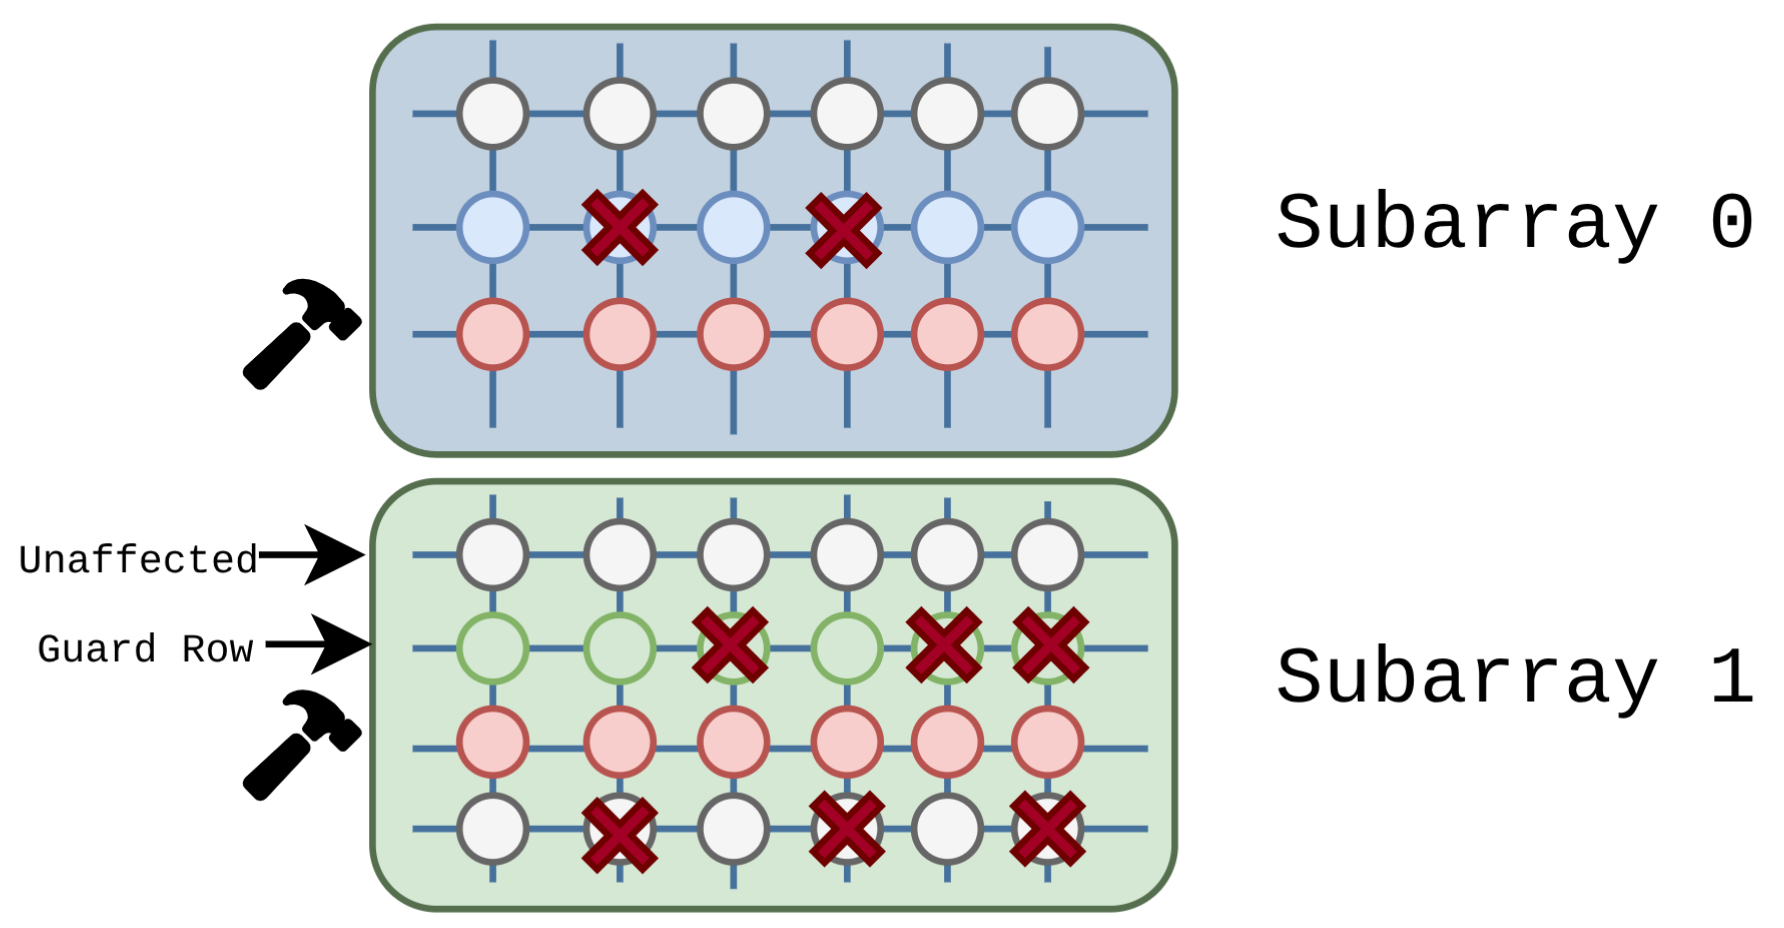
\includegraphics[width=\columnwidth]{isolation_colored.png}
	\caption{Isolation-centric mitigations based on partitioning. RowHammer cannot occur cross-subarray. Guard rows can be placed between aggressor rows and victim rows protect victims. There might be more than one guard rows in practice taking the blast radius into account.}\label{fig:isolation}
\end{figure}

Physical boundaries generally take two forms: \textit{guard rows}, and \textit{subarray isolation}, as illustrated by Fig. \ref{fig:isolation}. Guard rows are unused rows placed between potential aggressor and victim rows to "absorb" bit-flips. Due to the spatial locality of RowHammer effect, it is a lot harder for the aggressor row to induce bit-flips across all guard rows in between. The earliest partitioning approach, though not being a direct mitigation to RowHammer itself, was a bank-aware memory allocator proposed by \cite{Yun14}, which enables memory pages to be allocated to specific banks. Then, \cite{Brasser16} was the first to use guard rows to defend against RowHammer by placing one guard row between kernel space and user space, and between memory regions of any two processes. \cite{Izzo18} soon realized that one guard row was not sufficient to defeat increasingly sophisticated attack pattern, raising the number of guard rows to 8. Later, Konoth et al.\cite{Konoth18} proposed ZebRAM, placing one guard row between every two adjacent memory rows, thereby protecting the entire DRAM. While they claimed to use guard rows for integrity check and swap space, this essentially halved the memory space available for storing conventional data. Similarly, \cite{Tatar18,Bock19} also use guard rows to protect confidential data.

This trend presents a main controversy with partitioning: \textit{capacity loss}, memory space that is rendered unusable for guarding purpose. Meanwhile, \cite{Loughlin21} criticizes that these mitigations forgo \textit{Bank-Level Parallelism (BLP)}, an important performance optimization in modern DRAM. Since memory operations on different DRAM banks can be carried out concurrently, putting memory pages from a trust domain, such as a process, in a single bank risks creating a hot-bank and serializing all subsequent memory access to this domain.

Consequently, \cite{Loughlin21} stressed the importance of utilizing subarray isolation to restore BLP. That is, subarrays within the same bank are isolated from each other as they do not share bitlines, so hammering a row in a subarray will not affect an adjacent subarray (See Fig. \ref{fig:isolation}). Therefore, memory pages from a domain can still be placed in different banks while being isolated, as long as they are in not in the same subarray. Siloz\cite{Loughlin23} is a mitigation employing this strategy: it focuses on mitigating inter-VM RowHammer attacks by placing memory lines from different VMs in different subarrays, preventing RowHammer across trust domains (VMs). Unfortunately, it is criticized by \cite{Saxena24_2} for introducing \textit{stranding}, the second challenge of partitioning, which refers to DRAM space being underutilized, as space in a subarray cannot be used by other trust domains and might remain unused by the owner. \cite{Saxena24_2,M25} sought to further reduce stranding only strictly enforce isolation on confidential data.

Apart from using guard rows and subarray-isolation, there are other approaches to break spatial correlation. NoHammer\cite{Lee23} stores the memory lines of aggressors in an extended cache area, ensuring their memory lines are never evicted from the cache. Since a memory access cannot reach DRAM if the line it accesses is already in the cache, NoHammer prevents activation to aggressor rows in the DRAM, practically moving them into the cache.

The evolution of partitioning mitigation approaches, in my observation, reflects two fundamental design tradeoff. The tradeoff between domain-aware protection and universal protection, and between capacity loss and stranding. \cite{Yun14,Brasser16,Izzo18,Tatar18,Bock19,Loughlin23,Saxena24_2,M25} have only used guard rows to protect confidential data and isolate memory space from different trust domains, as defined by the memory allocator on the OS level, which creates a semantic gap: the underlying hardware has no knowledge to decide which rows are to be protected. Conversely, universal protections like ZebRAM\cite{Konoth18} do not rely on the knowledge of trust domains, but they give up the flexibility to selectively protect rows, which leads us to the next tradeoff. Capacity loss stems from using guard rows as scapegoats, in turns losing the ability to utilize part of the memory space, whereas stranding is a result of using physical boundaries in DRAM, like banks and subarrays. Nonetheless, granting a certain domain exclusive access to a memory region prevents using the area not occupied by it currently. It also raises scalability issue because the number of trust domains in scaled system can quickly exceeds the number of subarrays.

\subsubsection{Remapping}

Remapping-based mitigations break spatial proximity by changing the neighbor rows of potential aggressor rows, so that the attacker cannot reliably identify and target a sensitive victim row. They are either static or dynamic, depending on whether the remapping is determined upon initialization or adjusted during runtime. The early example of dynamic remapping includes \textit{Randomized Row-Swap (RRS)}\cite{Saileshwar22}, in which aggressor rows are identified using counters and swapped with another randomly selected row. \cite{Saxena22,Saxena24,Wi26} also proposed mitigations alike. Dynamic remapping has a common prerequisite of identifying aggressor rows, which is usually implemented with a refresh-centric mitigation. Therefore, Rubix\cite{Saxena24} acts as an enhancement to refresh-centric mitigation approaches, aiming to reduce the number of hot-rows.

\begin{figure}[h]
	\centering
	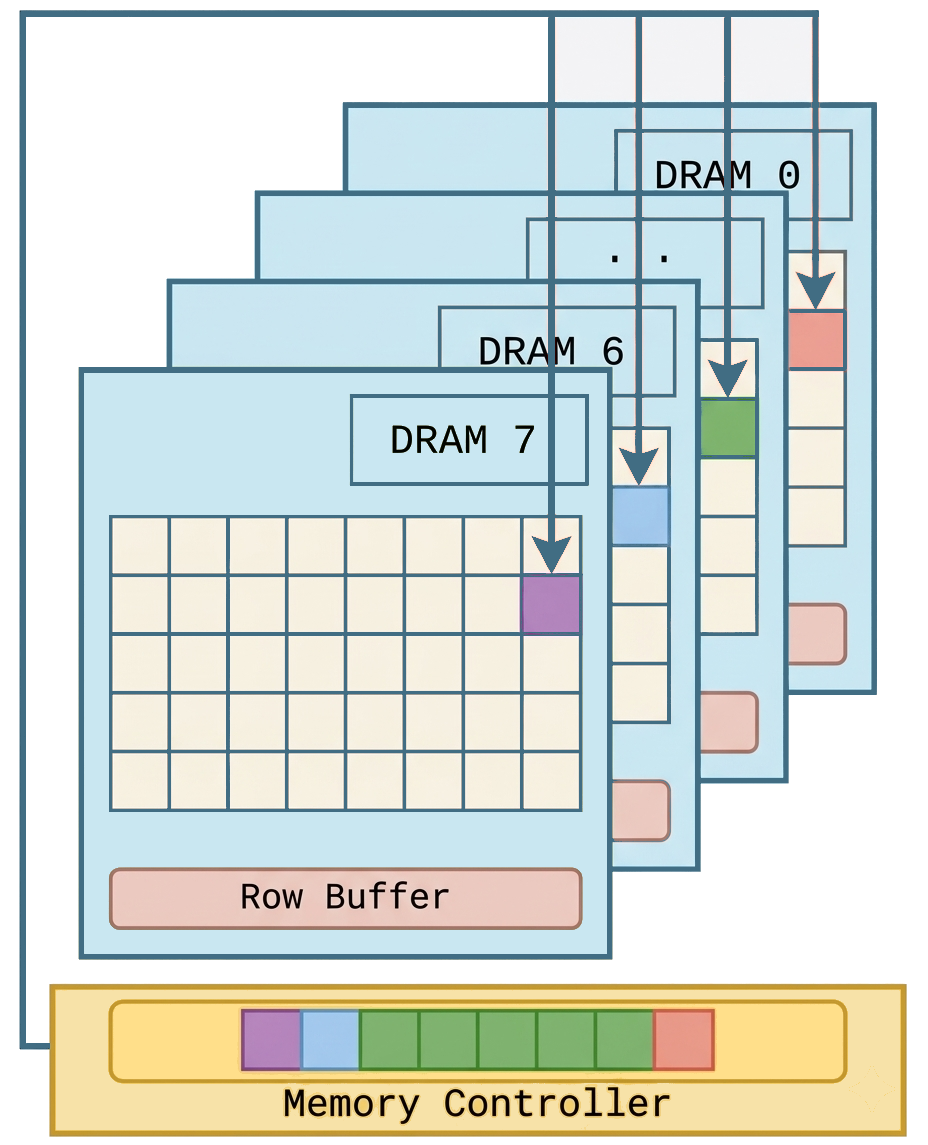
\includegraphics[width=0.7\columnwidth]{supercell_colored.png}
	\caption{A controller row is aggregated from cells with the same address in all DRAMs in the rank.}\label{fig:supercell}
\end{figure}

Dynamically shuffling rows can be expensive: it requires storing mapping relationships in precious SRAM space and incurs performance overhead for swapping rows. Static defenses, pioneered by RAMPART\cite{Woo24}, sought to address this issue. Woo et al. made the key observation that when a controller row is hammered, the corresponding address in all DRAM chips are affected because a controller row is aggregated from cells with the same address in each DRAM chip in the same bank (As shown in Fig. \ref{fig:supercell}). Accordingly, shuffling rows in each DRAM leads to errors being spread out in different logical rows. Noting that if the bit-flips are scattered in different rows, it is possible to restore the corrupted data by using \textit{Error-Correction Code (ECC)} such as \textit{Single Device Data Correction (SDDC)}, a mechanism in memory to correct data corruption. The combination of static remapping and ECC confront the attacker to defeat both of them simultaneously to produce bit-flips.

Remapping and partitioning mitigate RowHammer at the cost of spatial capacity and latency, respectively. The remapping-based mitigations are generally more transparent, eliminating the semantic gap between OS and hardware and providing universal protection that most partitioning mitigations forfeit for the sake of resource utilization, while partitioning offers a physical boundary that is easier to verify.

\section{Discussion}

\subsection{A Fundamental Assumption Failure}

The classical threat vector of RowHammer has evolved into a broader characterization of DRAM disturbance error. Specifically, RowPress\cite{Luo23} is a disturbance error pattern in which bit-flips occur near DRAM rows that are kept open (activated) for an extended period of time. \cite{Luo23} found that this phenomenon can substantially reduce RowHammer thresholds of nearby rows. In extreme cases, $T_{RH}$ can be decreased to as low as 1. RowPress can also cause bit-flips within a short period if combined with RowHammer\cite{Luo24_2}.  Section \ref{sec:prev-work} highlighted that all reactive mitigations, including refresh-centric, frequency-centric, and dynamic shuffling isolation-centric mitigation approaches, are based on the assumption that frequent activation to aggressor rows is a prerequisite of causing bit-flips. However, the introduction of RowPress renders this assumption completely invalid. Unless explicitly taking row open time into account, reactive mitigations expose DRAM to the threat of RowPress while seemingly protecting it. 

Granted, refresh-centric and frequency-centric mitigations are still prevalent because they are optimized for common cases, where $T_{TH}$ is far greater than 1, but RowPress reveals a deep research gap: factors that are known to influence RowHammer threshold, apart from activation count, are underappreciated.  \cite{Orosa21} identified that aggressor row active time is a key property that influences $T_{RH}$ back in 2021, and RowPress leverages this effect to break reactive mitigations in 2023. Factors that are proven to have an impact on $T_{RH}$, including temperature, victim DRAM cell's physical location, physical region of DRAM, wordline voltage, etc.\cite{Orosa21,Yaglikci22}. Although existing mitigations can be modified to prevent RowPress (e.g. \cite{Luo23,Luo24,Qureshi24_2}), this only addresses the specific mechanism RowPress exploits, not the broader class of underappreciated factors, so future attack variants can exploit said factors to bypass mitigations that are regarded as secure today. Therefore, security proofs for reactive mitigations should be regarded conditional on the assumption that activation count is the only disturbance variable, an assumption that has been proven false by RowPress and will be further weakened by other factors.

\subsection{The Scalability Crisis}

The exacerbating $T_{RH}$ in new DRAM devices severely affects all three types of mitigations. Refresh-centric and frequency-centric mitigations are directly influenced by this trend, \cite{Vittal25} shows that PRAC + ABO in DDR5 already leads to a 10\% slowdown on average at current $T_{RH}$. Extrapolating the trend of decreasing $T_{RH}$, we can predict that current refresh-centric and frequency-centric mitigations will cause prohibitive slowdown. Decreasing $T_{RH}$ will also overwhelm the mitigation policy of refresh-centric mitigations: unless combined with frequency-centric mitigations like ABO, only limited number of refresh can be carried out in a time window to ensure deterministic timing guarantees of DDR5\cite{Qureshi25}, so not all aggressor rows can be refreshed in a timely manner. Stateless refresh-centric mitigations based on probability also fall short on keeping up with low $T_{RH}$: they have to either set mitigation probability high to ensure security but adds high performance overhead, or set the probability very low to improve performance but erodes security.

Refresh-centric mitigations are further challenged by decreasing $T_{RH}$ as even refreshing itself becomes exploitable by attackers. \cite{Kogler22} demonstrated that it is possible to leverage the mitigative refresh operations as a secondary source of hammering, since refreshing is essentially reading and re-writing to a row, and excessive refresh operations also lead to excessive activations.

Isolation-centric mitigations that requires shuffling or quarantining aggressor rows suffer from decreasing $T_{RH}$ due to similar reasons. Other isolation-centric mitigations suffers from other scalability issues: increased blast radius and rapid growth of trust domains. While RowHammer is previously thought to influence only the immediate adjacent two rows (blast radius = 1), \cite{Kogler22} demonstrated that it is possible to hammer a row from next row over, leading to a blast radius of 2\cite{Marazzi23}. Increased blast radius requires more guard rows to be placed between memory space from different trust domains, leading to more space wasted. More trust domains will also leads to performance degradation: as the number of trust domains increases, more subarrays must be dedicated to them, leading to internal fragmentation, and isolating numerous domains into dedicated subarrays also limits bank-level parallelism can be exploited\cite{M25}.

Shrinking of $T_{RH}$ is pushing all current mitigations to a point where their performance overhead degrades availability. Though isolation-centric mitigations are utterly expensive as their storage overhead reduces capacity gained by scaling, static remapping or partitioning approaches are among the few ones that do not lead to significant additional slowdown as $T_{RH}$ falls. Hence, breaking spatial correlation instead of issuing mitigation operations might be useful to solving the scalability issue.

\subsection{Proven Insecure or Insecurely Proven: Access-Pattern Dependency}

Across all reactive defenses, a common tradeoff arises from whether making an informed mitigation decision or maintaining access-pattern independence. Access-pattern \cite{Frigo20} shows that carefully crafted attacks can deceive mitigations depending on access-pattern: it is  possible for attackers to frequently activate dummy rows to fill up the tracker array in many-sided attack, so dummy rows instead of actual aggressors are mitigated, rendering counting-based mitigation ineffective. 

Meanwhile, any mitigations whose observable behavior varies with access-pattern can enable a timing side-channel, an ubiquitous yet underappreciated issue actively considered by only very few works. Timing side-channels are a covert way to leak information that arises from physical properties. For example, an attacker can encode a bit by choosing whether or not to hammer a row (e.g. intentionally triggering RowHammer mitigation represents a ``1", and refraining represents a ``0"). On the receiving side, the attacker can infer the bit by observing the timing differences caused by RowHammer mitigation, such as when ABO in DDR5 slows down the memory controller upon an attack. Solutions to timing side-channel have been proposed, including a stateless refresh-centric mitigation, FR-RFM\cite{Bostanci25}, which periodically issues RFM regardless of access-pattern, and TPRAC\cite{Woo25} which randomly issues RFM to add noise to the side-channel. However, both of them add additional mitigation operations to existing ones, leading to performance overhead, and the latter does not completely disable the side-channel, but merely making it more costly for transmission.

Probabilistic refresh-centric mitigations are often seen as decoupled from access-pattern , hence not affected by timing side-channel. However, their major problem is that they are non-deterministic, so there is always a chance for a successful attack. Some studies mathematically prove that their probabilistic mitigations are secure, but they might still fall due to unforeseen attack variants or incorrect underlying assumptions, as supported by \cite{Anderson23}, which further argues that security proofs can be unreliable or misleading because of factors such as abstraction errors.

Access-pattern dependency introduces a central tension: either accepting an approach that is already proven insecure, risking enabling timing side-channel attacks or being deceived by many-sided attacks, or using probabilistic mitigations that appear secure but remain non-deterministic. Therefore, this dilemma cannot be resolved by reactive mitigations, leaving proactive mitigations that focus on prevention rather than reaction as a better choice.

\subsection{Evaluation Gap}

RowHammer research will benefit from a more uniform benchmark and evaluation framework. It was found that many papers choose different benchmarks to present the performance and security guarantee of their mitigations. which prevents direct comparison with other mitigations, A survey by Anderson and Boucher\cite{Heckel26_2} also raises questions about the general validity of some RowHammer studies, many of which uses a small sample size and yield results not comparable with other studies. Therefore, building a uniform framework for mitigation analysis is urgently needed so that the field can reach a consensus on the effectiveness of mitigations.

\subsection{Limitations of This Study}

This study puts an emphasis on those proposed after 2023, so some older mitigations might be underrepresented.  Though this study aims to be comprehensive, it is not necessarily exhaustive. To emphasize the tradeoffs in design choices, this study described many mitigations in a simplified manner, omitting some details of implementation, and did not include quantitative analysis.

\section{Conclusion}

\begin{figure}[h]
	\centering
	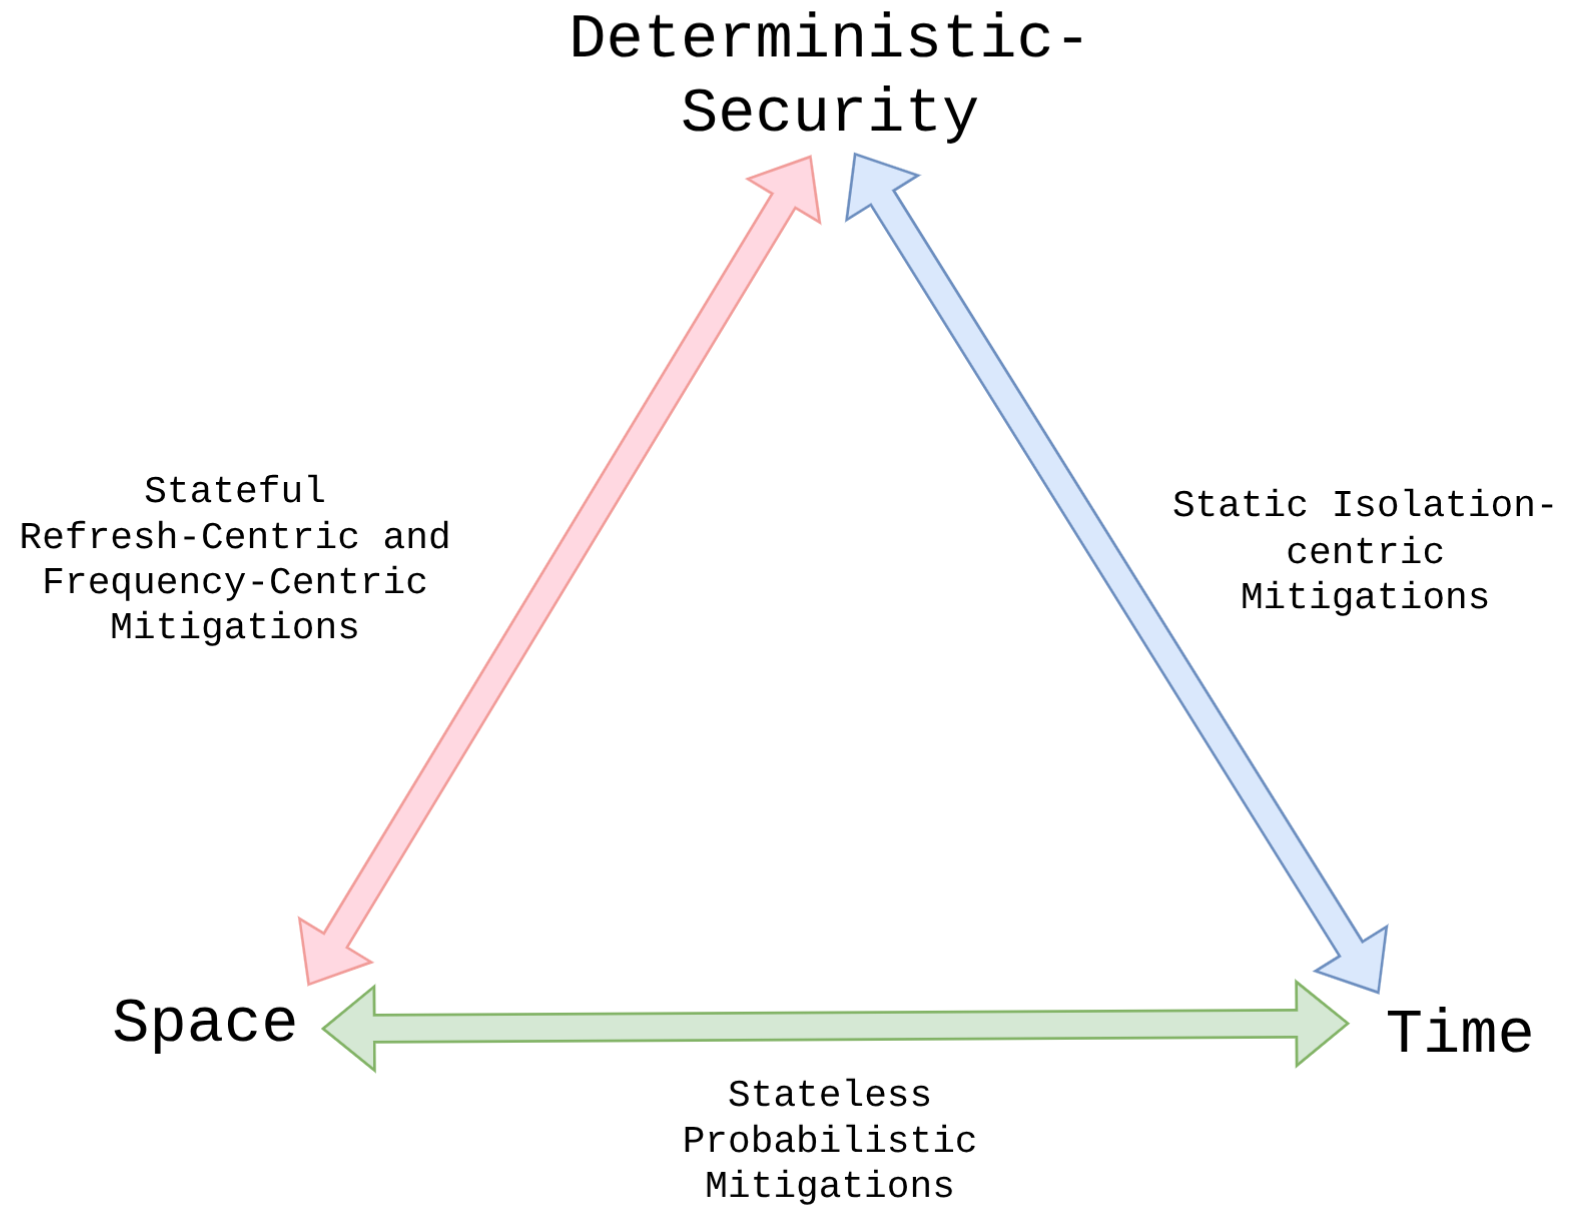
\includegraphics[width=\columnwidth]{unholytri.png}
	\caption{The impossible trinity: none of current mitigations can be efficient in space and time while guarantee deterministic-security. Mitigations on each edge forgo the advantage indicated at the opposite node.}\label{fig:unholy}
\end{figure}

This study surveys RowHammer mitigations and classify them into three groups: refresh-centric, frequency-centric, and isolation-centric, and further categorize mitigations in each group to analyze their design tradeoffs. In this study, the taxonomy proposed in Loughlin et al.'s 2021 paper\cite{Loughlin21} is employed for classification. However, some defenses fit in multiple categories, rendering the taxonomy not mutually exclusive. This study proposes that this observation shows the necessity to take a hybrid approach to combine the strengths of multiple types of mitigations. By considering the common strength and downsides of each group of mitigations, this study further concludes that current mitigations cannot simultaneously fulfill space-efficiency, low-latency, and deterministic-security (as illustrated in Fig. \ref{fig:unholy}). Understanding the inherent trade-offs in current defenses is essential for guiding the design of the next generation of robust and efficient memory protection mechanisms. 

\bibliographystyle{IEEEtran}
\hypersetup{hidelinks,pdfborder={0 0 0},breaklinks=true}
\bibliography{refs}
\end{document}